%!TEX TS-program = xelatex

% HSE Beamer Theme
% by Danil Fedorovykh
% http://hse.ru/staff/df
%
% Version 2.0 (English)
% January 2022

%%% Set up the free HSE Sans font
%%% https://www.hse.ru/info/brandbook/#font

\documentclass[aspectratio=169]{beamer}

\newbool{russian}
\booltrue{russian} % Uncomment if in Russian
\usepackage{HSE-theme/beamerthemeHSE} % Load HSE theme
\usepackage[no-math]{fontspec}      % fonts loading
\usepackage{caption}
\usepackage{subfigure}
\usepackage{subcaption}
\usepackage{hyperref}
\usepackage[dvipsnames]{xcolor}
\usepackage{ragged2e}
\captionsetup[figure]{labelformat=empty}
\captionsetup[subfigure]{labelformat=empty}
\renewcommand*{\thesubfigure}{(\arabic{subfigure})}
\setsansfont{HSE Sans}
%\graphicspath{{./images/}}
\graphicspath{{/home/llyy/Yandex.Disk/personal/knowledge/general/algorithms_course/repo/algorithms_course/4_search/lection/images}}


%%% Информация об авторе и выступлении
\title[Title]{Алгоритмы и структуры данных} 
\subtitle{Лекция 4. Алгоритмы поиска}
\author[Author's name]{Илья Сергеевич Бычков\\ \smallskip \scriptsize \url{ibychkov@hse.ru}}
\institute{НИУ ВШЭ - Нижний Новгород}
\date{\today}


\begin{document}

\frame[plain]{\titlepage}

%%%%%%%%%%%%%%%%%%%%%%%%%%%%%%%%%%%%%%%%%%%%%%%%%%%%%%%%%%%%%%%%%%%%%%%%%%%%%%%%%%%%%%%%%%%%%%%%%%
\begin{frame}[c]
%\frametitle{A first slide}

\begin{center}
\Huge Лекция 4.

\Huge Алгоритмы поиска
\end{center}

\end{frame}

%%%%%%%%%%%%%%%%%%%%%%%%%%%%%%%%%%%%%%%%%%%%%%%%%%%%%%%%%%%%%%%%%%%%%%%%%%%%%%%%%%%%%%%%%%%%%%%%%%
\begin{frame}
\frametitle{Алгоритмы поиска}
\framesubtitle{План лекции}

\begin{enumerate}
  \setcounter{enumi}{-1}
  \item{План лекции}
  \item{\textcolor{blue}{Задача поиска}}
  \item{Линейный поиск}
  \item{Двоичный/бинарный поиск}
  \item{Троичный/тернарный поиск}
  \item{Экспоненциальный поиск}
  \item{Интерполяционный поиск}
  \item{Jump поиск}
\end{enumerate}
\end{frame}



%%%%%%%%%%%%%%%%%%%%%%%%%%%%%%%%%%%%%%%%%%%%%%%%%%%%%%%%%%%%%%%%%%%%%%%%%%%%%%%%%%%%%%%%%%%%%%%%%%
\begin{frame}
\frametitle{Задача поиска}
\framesubtitle{Задача поиска}
\justifying
\textcolor{red}{Задача поиска} заключается в нахождении объектов с заданными свойствами среди конечного количества объектов.
\newline\newline
\textcolor{blue}{Входные данные}: коллекция/контейнер с объектами, искомый критерий \newline (функция/предикат)\newline\newline
\textcolor{blue}{Выходные данные}: информация о местоположении искомых объектов в коллекции (обычно индекс или набор индексов)\newline\newline
Задача поиска является самой фундаментальной задачей в области компьютерных наук.
\end{frame}


%%%%%%%%%%%%%%%%%%%%%%%%%%%%%%%%%%%%%%%%%%%%%%%%%%%%%%%%%%%%%%%%%%%%%%%%%%%%%%%%%%%%%%%%%%%%%%%%%%
\begin{frame}
\frametitle{Алгоритмы поиска}
\framesubtitle{План лекции}

\begin{enumerate}
  \setcounter{enumi}{-1}
  \item{План лекции}
  \item{Задача поиска}
  \item{\textcolor{blue}{Линейный поиск}}
  \item{Двоичный/бинарный поиск}
  \item{Троичный/тернарный поиск}
  \item{Экспоненциальный поиск}
  \item{Интерполяционный поиск}
  \item{Jump поиск}
\end{enumerate}
\end{frame}


%%%%%%%%%%%%%%%%%%%%%%%%%%%%%%%%%%%%%%%%%%%%%%%%%%%%%%%%%%%%%%%%%%%%%%%%%%%%%%%%%%%%%%%%%%%%%%%%%%
\begin{frame}
\frametitle{Линейный поиск}
\framesubtitle{Линейный поиск}
\justifying
\textcolor{red}{Линейный поиск (linear search)} — простейший алгоритм поиска (полный перебор).\newline\newline Заключается в последовательной проверке каждого элемента коллекции на \newline соответствие заданному критерию поиска. \newline\newline Алгоритм выполняется пока не будет найдено совпадение(или все совпадения) или не будут проверены все элементы.

\begin{figure}
    \captionsetup[subfigure]{labelformat=empty}
    \centering
    \subfigure[{ \scriptsize Линейный поиск (linear search), Источник - \href{https://www.geeksforgeeks.org/linear-search/}{Geeks4Geeks}}]{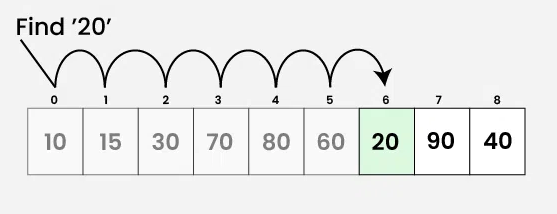
\includegraphics[width=75mm, height=28mm]{linear_search}} 
\end{figure}
\end{frame}

%%%%%%%%%%%%%%%%%%%%%%%%%%%%%%%%%%%%%%%%%%%%%%%%%%%%%%%%%%%%%%%%%%%%%%%%%%%%%%%%%%%%%%%%%%%%%%%%%%
\begin{frame}
\frametitle{Линейный поиск}
\framesubtitle{Линейный поиск}
\justifying
\textcolor{red}{Линейный поиск (linear search)} \newline\newline
Преимущества:\newline
\textcolor{green} {\textbf{+}} крайне прост в реализации\newline
\textcolor{green} {\textbf{+}} может работать без какой-либо дополнительной информации о данных\newline\newline
Недостатки:\newline
\textcolor{red} {\textbf{-}} линейная сложность $\mathcal{O}(n)$ по времени в худшем и среднем случаях\newline

Алгоритм использует константный размер дополнительной памяти $\mathcal{O}(1)$. \newline Однако, это является общим свойством для большинства алгоритмов поиска.
\end{frame}

%%%%%%%%%%%%%%%%%%%%%%%%%%%%%%%%%%%%%%%%%%%%%%%%%%%%%%%%%%%%%%%%%%%%%%%%%%%%%%%%%%%%%%%%%%%%%%%%%%
\begin{frame}
\frametitle{Алгоритмы поиска}
\framesubtitle{План лекции}

\begin{enumerate}
  \setcounter{enumi}{-1}
  \item{План лекции}
  \item{Задача поиска}
  \item{Линейный поиск}
  \item{\textcolor{blue}{Двоичный/бинарный поиск}}
  \item{Троичный/тернарный поиск}
  \item{Экспоненциальный поиск}
  \item{Интерполяционный поиск}
  \item{Jump поиск}
\end{enumerate}
\end{frame}

%%%%%%%%%%%%%%%%%%%%%%%%%%%%%%%%%%%%%%%%%%%%%%%%%%%%%%%%%%%%%%%%%%%%%%%%%%%%%%%%%%%%%%%%%%%%%%%%%%
\begin{frame}
\frametitle{Двоичный/бинарный поиск}
\framesubtitle{Двоичный/бинарный поиск}
\justifying
\textcolor{red}{Двоичный/бинарный поиск (binary search)} — классический алгоритм поиска элемента в \textcolor{blue}{отсортированном} массиве.\newline\newline Делит текущий рассматриваемый интервал альтернатив на 2 половины. В зависимости от значения элемента в середине интервала рекурсивно решает такую же подзадачу для левой половины или для правой.


\begin{figure}
    \captionsetup[subfigure]{labelformat=empty}
    \centering
    \subfigure[{ \scriptsize Двоичный поиск (binary search), Источник - \href{https://www.geeksforgeeks.org/linear-search-vs-binary-search/}{Geeks4Geeks}}]{\includegraphics[width=115mm, height=35mm]{binary_search}}  
\end{figure}
\end{frame}

%%%%%%%%%%%%%%%%%%%%%%%%%%%%%%%%%%%%%%%%%%%%%%%%%%%%%%%%%%%%%%%%%%%%%%%%%%%%%%%%%%%%%%%%%%%%%%%%%%
\begin{frame}
\frametitle{Двоичный/бинарный поиск}
\framesubtitle{Двоичный/бинарный поиск}
\justifying
\textcolor{red}{Двоичный/бинарный поиск (binary search)}
\begin{figure}
    \captionsetup[subfigure]{labelformat=empty}
    \centering
    \subfigure[{ \scriptsize Реализация - \href{https://www.geeksforgeeks.org/binary-search/}{Geeks4Geeks}}]{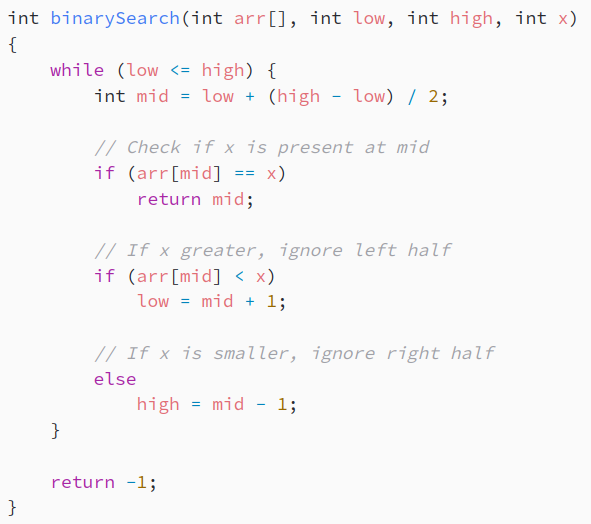
\includegraphics[width=60mm, height=59mm]{bs_iterative_c_impl}} 
    \subfigure[{ \scriptsize Реализация - \href{https://www.geeksforgeeks.org/binary-search/}{Geeks4Geeks}}]{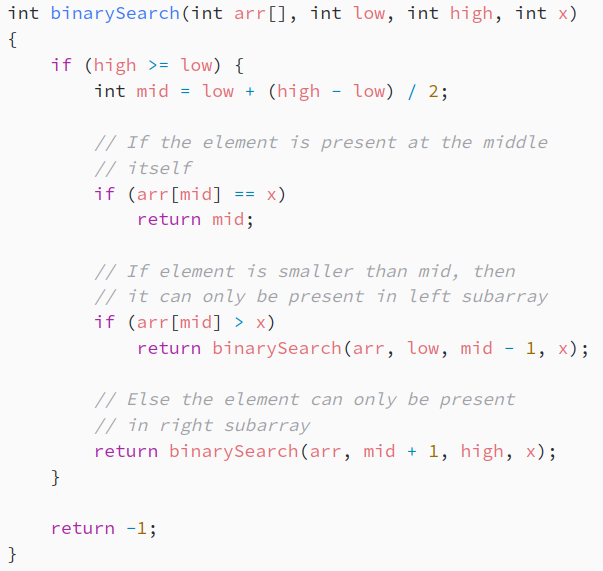
\includegraphics[width=60mm, height=59mm]{bs_recursive_c_impl}} 
\end{figure}
\end{frame}

%%%%%%%%%%%%%%%%%%%%%%%%%%%%%%%%%%%%%%%%%%%%%%%%%%%%%%%%%%%%%%%%%%%%%%%%%%%%%%%%%%%%%%%%%%%%%%%%%
\begin{frame}
\frametitle{Двоичный/бинарный поиск}
\framesubtitle{Двоичный/бинарный поиск}
\begin{block}{}
\begin{columns}[]
\column{\dimexpr\linewidth-30mm}

Преимущества:\newline
\textcolor{green} {\textbf{+}} наиболее эффективный алгоритм для поиска\newline
\textcolor{green} {\textbf{+}} сложность по времени $\mathcal{O}(log_2 n)$\newline
\textcolor{green} {\textbf{+}} сложность по памяти $\mathcal{O}(1)$ в случае итеративной релизации\newline\newline
Недостатки:\newline
\textcolor{red} {\textbf{-}} сложность в реализации\newline
\textcolor{red} {\textbf{-}} требование к данным - предварительная сортировка \newline
\textcolor{red} {\textbf{-}} требование к коллекции - эффективная операция произвольного доступа \newline

\column{35mm}
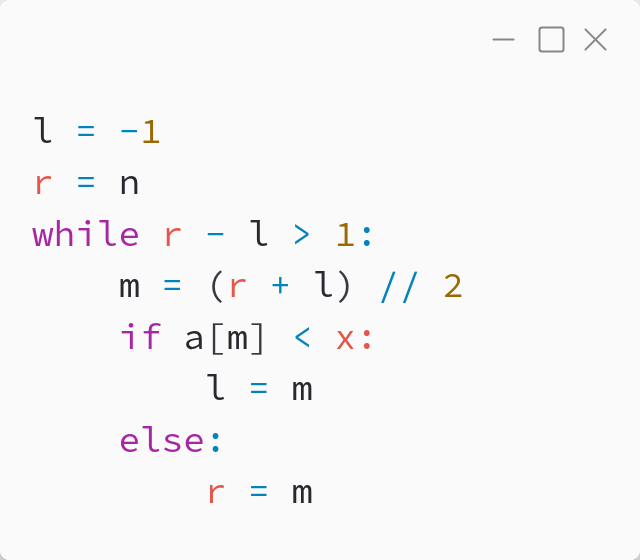
\includegraphics[width=35mm, height=30mm]{bs_pseudo_iter}
\center \tiny Реализация - \href{https://notes.algoprog.ru/binsearch/07_binsearch_main.html}{Algoprog}


\end{columns}
\end{block}
\end{frame}


%%%%%%%%%%%%%%%%%%%%%%%%%%%%%%%%%%%%%%%%%%%%%%%%%%%%%%%%%%%%%%%%%%%%%%%%%%%%%%%%%%%%%%%%%%%%%%%%%%
\begin{frame}
\frametitle{Двоичный/бинарный поиск}
\framesubtitle{Двоичный поиск по ответу}
\justifying
\textcolor{blue}{Задача}\newline\newline
В лабиринте есть $n$ комнат. В каждой комнате есть монстр, сила которого равна $a_i$. Игрок может использовать магию, чтобы уничтожить монстра силой $P$, но она действует только на монстров силой $\leq P$. Найти минимальную силу $P$, чтобы за одну атаку уничтожить как минимум $k$ монстров.

\begin{figure}
    \captionsetup[subfigure]{labelformat=empty}
    \centering
    \subfigure[{Известный мем}]{
\includegraphics[width=70mm, height=35mm]{monsters_meme}} 
   
\end{figure}
\end{frame}

%%%%%%%%%%%%%%%%%%%%%%%%%%%%%%%%%%%%%%%%%%%%%%%%%%%%%%%%%%%%%%%%%%%%%%%%%%%%%%%%%%%%%%%%%%%%%%%%%%
\begin{frame}
\frametitle{Алгоритмы поиска}
\framesubtitle{План лекции}

\begin{enumerate}
  \setcounter{enumi}{-1}
  \item{План лекции}
  \item{Задача поиска}
  \item{Линейный поиск}
  \item{Двоичный/бинарный поиск}
  \item{\textcolor{blue}{Троичный/тернарный поиск}}
  \item{Экспоненциальный поиск}
  \item{Интерполяционный поиск}
  \item{Jump поиск}
\end{enumerate}
\end{frame}

%%%%%%%%%%%%%%%%%%%%%%%%%%%%%%%%%%%%%%%%%%%%%%%%%%%%%%%%%%%%%%%%%%%%%%%%%%%%%%%%%%%%%%%%%%%%%%%%%%
\begin{frame}
\frametitle{Троичный/тернарный поиск}
\framesubtitle{Троичный/тернарный поиск}
\justifying
\textcolor{red}{Троичный/тернарный поиск (ternary search)} — алгоритм поиска минимума или \newline максимума функции на отрезке, которая либо сначала строго возрастает, затем строго убывает, либо наоборот. 

\begin{figure}
    \captionsetup[subfigure]{labelformat=empty}
    \centering
    \subfigure[{ \scriptsize Троичный поиск - \href{https://neerc.ifmo.ru/wiki/index.php?title=Троичный_поиск}{ИТМО}}]{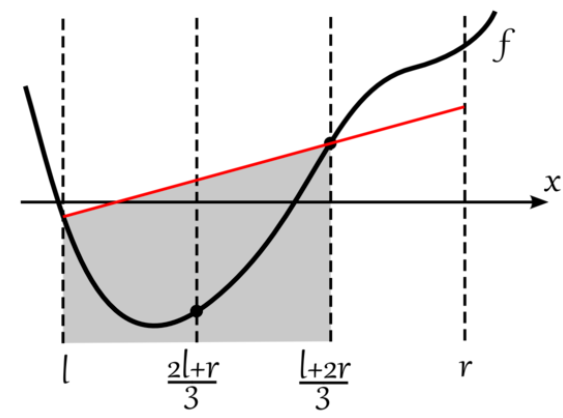
\includegraphics[width=60mm, height=40mm]{ternary}} 
\end{figure}
\end{frame}

%%%%%%%%%%%%%%%%%%%%%%%%%%%%%%%%%%%%%%%%%%%%%%%%%%%%%%%%%%%%%%%%%%%%%%%%%%%%%%%%%%%%%%%%%%%%%%%%%%
\begin{frame}
\frametitle{Троичный/тернарный поиск}
\framesubtitle{Троичный/тернарный поиск}
\justifying
\textcolor{red}{Троичный/тернарный поиск (ternary search)}\newline\newline
Итеративный вариант

\begin{figure}
    \captionsetup[subfigure]{labelformat=empty}
    \centering
    \subfigure[{ \scriptsize Троичный поиск - \href{https://neerc.ifmo.ru/wiki/index.php?title=Троичный_поиск}{ИТМО}}]{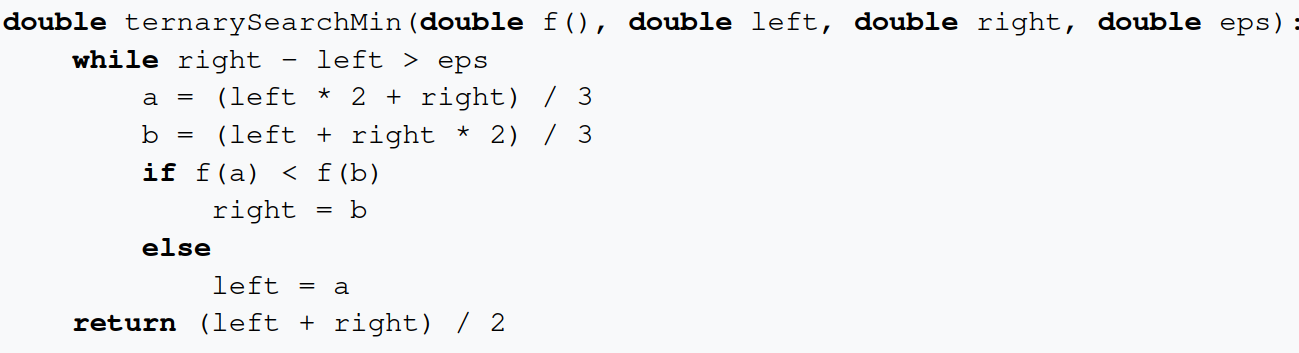
\includegraphics[width=130mm, height=40mm]{ternary_iterative}} 
\end{figure}
\end{frame}

%%%%%%%%%%%%%%%%%%%%%%%%%%%%%%%%%%%%%%%%%%%%%%%%%%%%%%%%%%%%%%%%%%%%%%%%%%%%%%%%%%%%%%%%%%%%%%%%%%
\begin{frame}
\frametitle{Троичный/тернарный поиск}
\framesubtitle{Троичный/тернарный поиск}
\justifying
\textcolor{red}{Троичный/тернарный поиск (ternary search)}\newline\newline
Итеративный вариант

\begin{figure}
    \captionsetup[subfigure]{labelformat=empty}
    \centering
    \subfigure[{ \scriptsize Троичный поиск - \href{https://neerc.ifmo.ru/wiki/index.php?title=Троичный_поиск}{ИТМО}}]{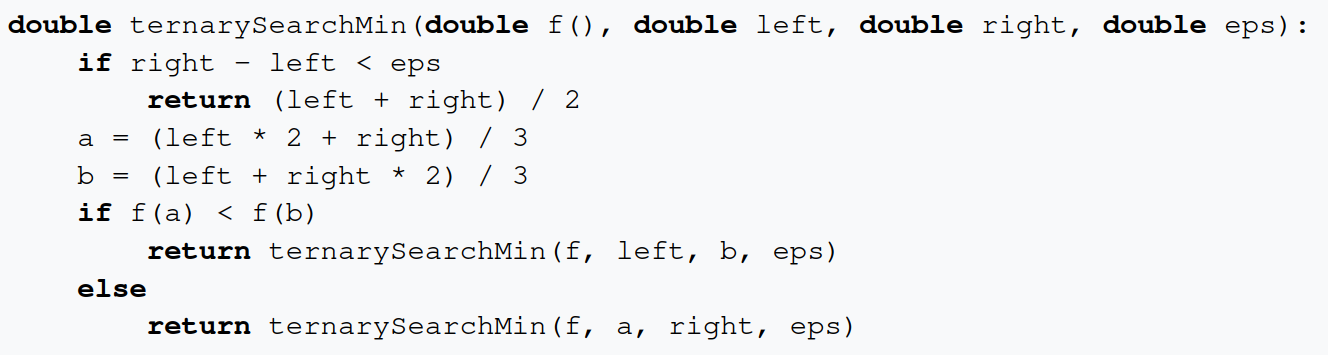
\includegraphics[width=130mm, height=40mm]{ternary_recursive}} 
\end{figure}
\end{frame}

%%%%%%%%%%%%%%%%%%%%%%%%%%%%%%%%%%%%%%%%%%%%%%%%%%%%%%%%%%%%%%%%%%%%%%%%%%%%%%%%%%%%%%%%%%%%%%%%%%
\begin{frame}
\frametitle{Алгоритмы поиска}
\framesubtitle{План лекции}

\begin{enumerate}
  \setcounter{enumi}{-1}
  \item{План лекции}
  \item{Задача поиска}
  \item{Линейный поиск}
  \item{Двоичный/бинарный поиск}
  \item{Троичный/тернарный поиск}
  \item{\textcolor{blue}{Экспоненциальный поиск}}
  \item{Интерполяционный поиск}
  \item{Jump поиск}
\end{enumerate}
\end{frame}


%%%%%%%%%%%%%%%%%%%%%%%%%%%%%%%%%%%%%%%%%%%%%%%%%%%%%%%%%%%%%%%%%%%%%%%%%%%%%%%%%%%%%%%%%%%%%%%%%%
\begin{frame}
\frametitle{Экспоненциальный поиск}
\framesubtitle{Экспоненциальный поиск}
\justifying

\textcolor{red}{Экспоненциальный поиск (exponential/doubling/galloping search)} \newline Алгоритм поиска, используемый для поиска в отсортированных массивах. \newline Идея состоит в том, чтобы определить диапазон, в котором находится целевое значение, и выполнить бинарный поиск в пределах этого диапазона. 

\begin{figure}
    \captionsetup[subfigure]{labelformat=empty}
    \centering
    \subfigure[{ \scriptsize Экспоненциальный поиск - \href{https://www.chegg.com/homework-help/questions-and-answers/code-needed-python-firstrepeat-function-works-runs-o-log-r-lastrepeat-functions-works-run--q58541804}{Источник}}]{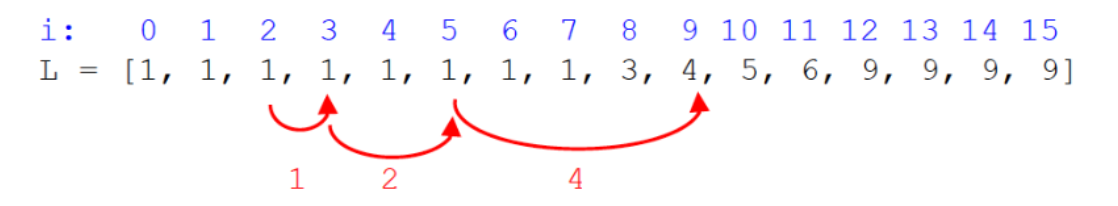
\includegraphics[width=130mm, height=20mm]{doubling}} 
\end{figure}

\end{frame}

%%%%%%%%%%%%%%%%%%%%%%%%%%%%%%%%%%%%%%%%%%%%%%%%%%%%%%%%%%%%%%%%%%%%%%%%%%%%%%%%%%%%%%%%%%%%%%%%%%
\begin{frame}
\frametitle{Экспоненциальный поиск}
\framesubtitle{Экспоненциальный поиск}
\justifying

\textcolor{red}{Экспоненциальный поиск (exponential/doubling/galloping search)}
\begin{figure}
    \captionsetup[subfigure]{labelformat=empty}
    \centering
    \subfigure[{ \scriptsize Экспоненциальный поиск - \href{https://en.wikipedia.org/wiki/Exponential_search}{Wiki}}]{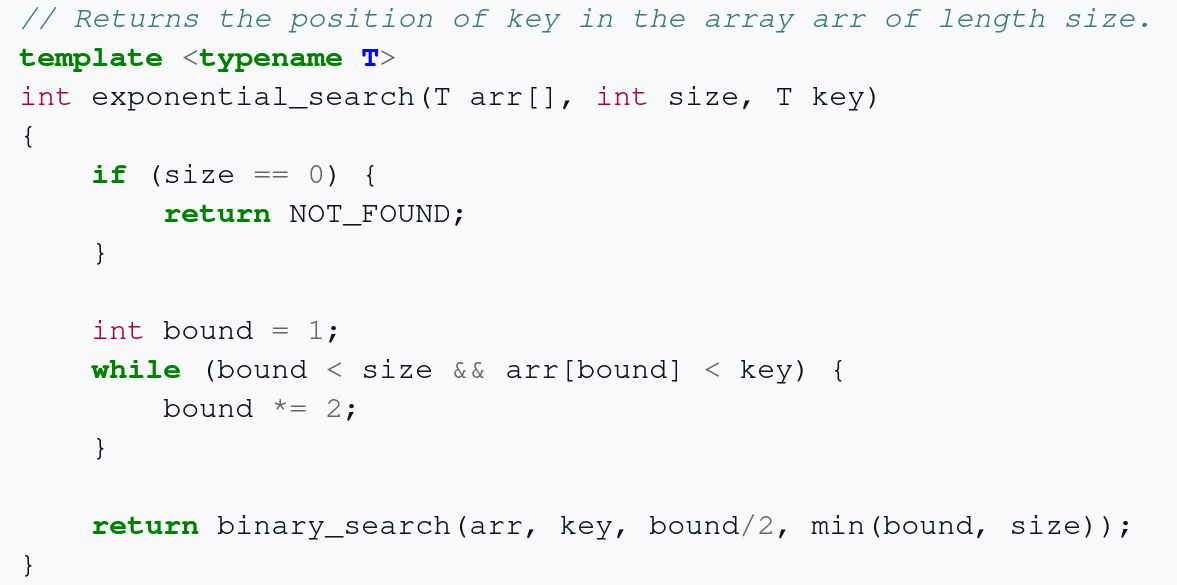
\includegraphics[width=80mm, height=40mm]{doubling_pseudo}}
    \subfigure[{ \scriptsize Сложность - \href{https://en.wikipedia.org/wiki/Exponential_search}{Wiki}}]{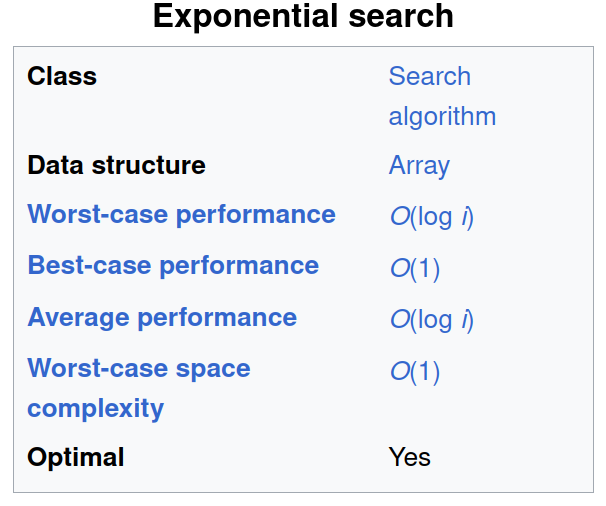
\includegraphics[width=40mm, height=30mm]{doubling_complexity}} 
\end{figure}

\end{frame}

%%%%%%%%%%%%%%%%%%%%%%%%%%%%%%%%%%%%%%%%%%%%%%%%%%%%%%%%%%%%%%%%%%%%%%%%%%%%%%%%%%%%%%%%%%%%%%%%%%
\begin{frame}
\frametitle{Алгоритмы поиска}
\framesubtitle{План лекции}

\begin{enumerate}
  \setcounter{enumi}{-1}
  \item{План лекции}
  \item{Задача поиска}
  \item{Линейный поиск}
  \item{Двоичный/бинарный поиск}
  \item{Троичный/тернарный поиск}
  \item{Экспоненциальный поиск}
  \item{\textcolor{blue}{Интерполяционный поиск}}
  \item{Jump поиск}
\end{enumerate}
\end{frame}

%%%%%%%%%%%%%%%%%%%%%%%%%%%%%%%%%%%%%%%%%%%%%%%%%%%%%%%%%%%%%%%%%%%%%%%%%%%%%%%%%%%%%%%%%%%%%%%%%%
\begin{frame}
\frametitle{Интерполяционный поиск}
\framesubtitle{Интерполяционный поиск}
\justifying
\textcolor{red}{Интерполяционный поиск (interpolation search)} — алгоритм поиска, который \newline используется для нахождения элемента в отсортированном массиве данных. \newline\newline Основан на предположении, что элементы массива распределены равномерно и что искомый элемент можно найти, используя линейную интерполяцию между двумя известными элементами массива.

\begin{figure}
    \captionsetup[subfigure]{labelformat=empty}
    \centering
    \subfigure[{ \scriptsize Индекс искомого элемента - \href{https://www.geeksforgeeks.org/interpolation-search-in-python/}{Geeks4Geeks}}]{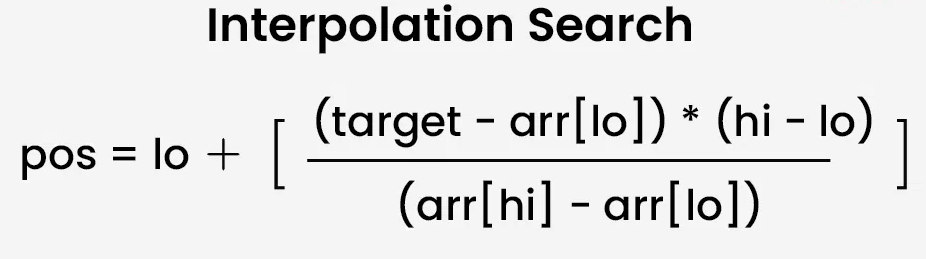
\includegraphics[width=100mm, height=30mm]{interpolation_formula}} 
\end{figure}

\end{frame}

%%%%%%%%%%%%%%%%%%%%%%%%%%%%%%%%%%%%%%%%%%%%%%%%%%%%%%%%%%%%%%%%%%%%%%%%%%%%%%%%%%%%%%%%%%%%%%%%%%
\begin{frame}
\frametitle{Интерполяционный поиск}
\framesubtitle{Интерполяционный поиск}
\justifying
\textcolor{red}{Интерполяционный поиск (interpolation search)}

\begin{figure}
    \captionsetup[subfigure]{labelformat=empty}
    \centering
    \subfigure[{ \scriptsize Интерполяционный поиск - \href{https://www.geeksforgeeks.org/interpolation-search-in-python/}{Geeks4Geeks}}]{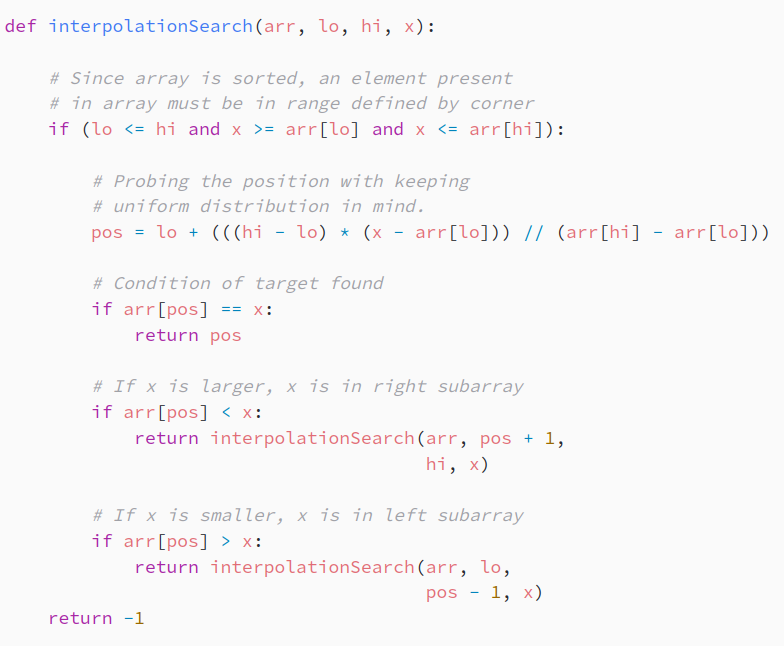
\includegraphics[width=70mm, height=59mm]{interpolation_pseudo}} 
\end{figure}

\end{frame}

%%%%%%%%%%%%%%%%%%%%%%%%%%%%%%%%%%%%%%%%%%%%%%%%%%%%%%%%%%%%%%%%%%%%%%%%%%%%%%%%%%%%%%%%%%%%%%%%%%
\begin{frame}
\frametitle{Алгоритмы поиска}
\framesubtitle{План лекции}

\begin{enumerate}
  \setcounter{enumi}{-1}
  \item{План лекции}
  \item{Задача поиска}
  \item{Линейный поиск}
  \item{Двоичный/бинарный поиск}
  \item{Троичный/тернарный поиск}
  \item{Экспоненциальный поиск}
  \item{Интерполяционный поиск}
  \item{\textcolor{blue}{Jump поиск}}
\end{enumerate}
\end{frame}

%%%%%%%%%%%%%%%%%%%%%%%%%%%%%%%%%%%%%%%%%%%%%%%%%%%%%%%%%%%%%%%%%%%%%%%%%%%%%%%%%%%%%%%%%%%%%%%%%%
\begin{frame}
\frametitle{Jump поиск}
\framesubtitle{Jump поиск}
\justifying
\textcolor{red}{Jump поиск (jump search)} — алгоритм поиска, который используется для нахождения элемента в отсортированном массиве данных. \newline\newline Основывается на более быстром (по отношению к линейному поиску) переборе элементов и поиске интервала, на котором расположен искомый элемент.

\begin{figure}
    \captionsetup[subfigure]{labelformat=empty}
    \centering
    \subfigure[{ \scriptsize Jump search - \href{http://theoryofprogramming.azurewebsites.net/2016/11/10/jump-search-algorithm/}{Источник}}]{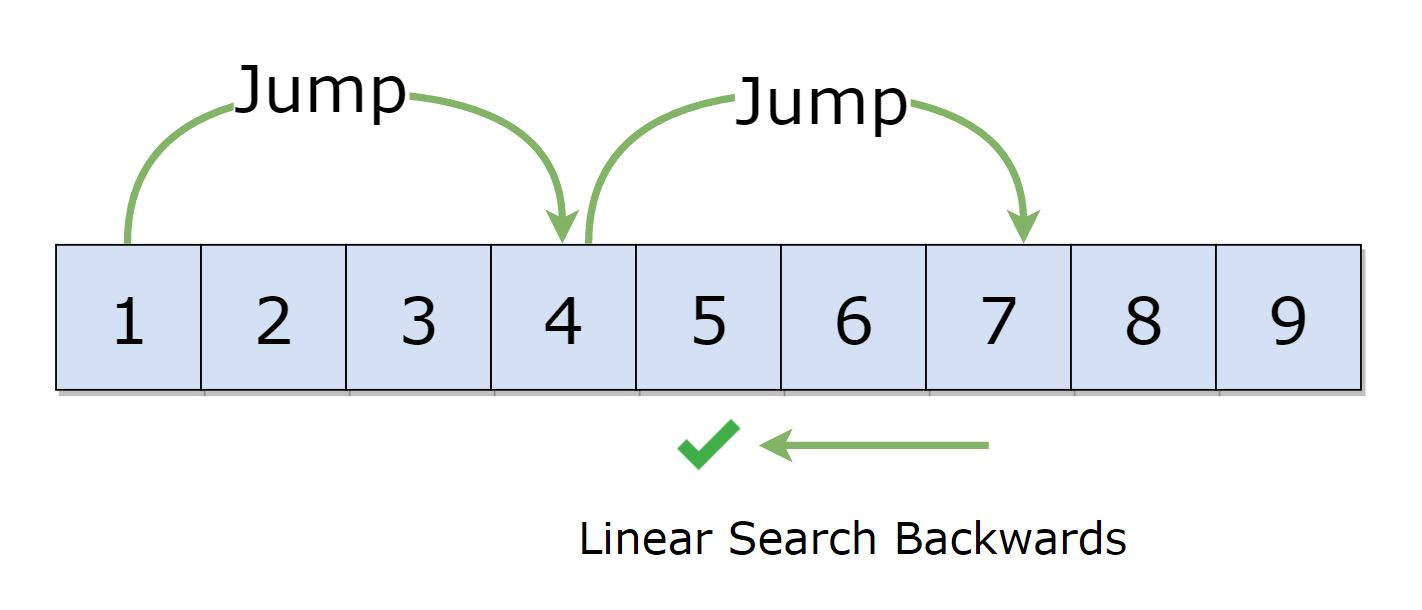
\includegraphics[width=90mm, height=30mm]{jump_search}} 
\end{figure}
\end{frame}

\end{document}